\chapter{Einleitung}

\par
In \cite{kato_1954}
%[\textsc{Kato}: \textit{On the semi-groups generated by Kolmogoroff's differential equations}. Journal of the Mathematical Society of Japan, 1954] 
zeigt \textsc{T. Kato} die Existenz einer $C_0$-Halbgruppe, welche das Kolmogorov'sche Differentialgleichungssystem eines Geburts- und Todesprozesses in $\ell^1$ löst. Das Ergebnis wurde u. a. von \textsc{J. Voigt} in \cite{voigt_1989} %[\textsc{Voigt}: \textit{On resolvent positive operators and positive $C_0$-semigroups on AL-spaces}. Semigroup Forum, 1989] 
auf die Klasse der AL-Räume erweitert, welche die Banachverbände  $\ell^1$ und $\text{L}^1(\Omega,\mu)$ umfasst.
\par
In dieser Arbeit wird das Ergebnis von \textsc{J. Banasiak} et al. in \cite{banasiak_lachowicz_2007}
%[\textsc{Banasiak, Lachowicz}: \textit{Around the Kato generation theorem for semigroups}. Studia Mathematica, 2007] 
vorgestellt, welches die Existenz von Lösungen auf die Klasse der KB-Räume verallgemeinert. Diese umfasst neben den AL-Räumen auch die reflexiven Banachverbände $\ell^p$ und $\text{L}^p(\Omega,\mu)$. 
\par
% \vspace{30px}
% \begin{figure}
%     \centering
%     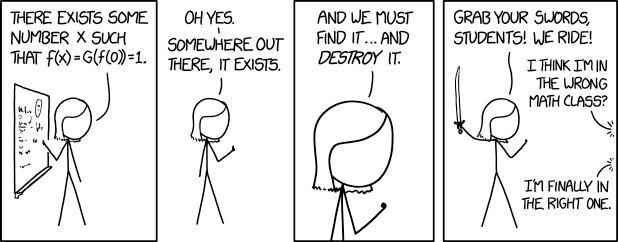
\includegraphics[scale = 0.55]{existence_proof}
%     \caption{\textsc{Existence Proof} (\textit{https://xkcd.com/1856/})}
% \end{figure}


% 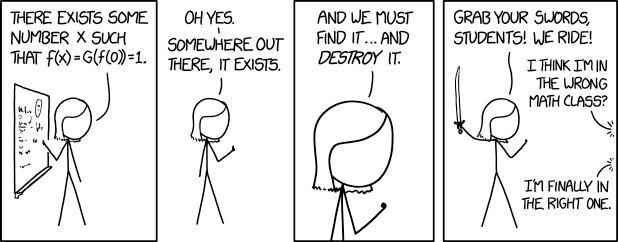
\includegraphics[scale = 0.55]{existence_proof}

% An dieser Stelle steht eine Zusammenfassung der Arbeit, Umfang
% max.\ 1 Seite. Im Unterschied zu anderen Kapiteln ist die
% Kurzfassung (und das Abstract) üblicherweise nicht in Abschnitte
% und Unterabschnitte gegliedert. 
% Auch Fußnoten sind hier falsch am Platz.

% Kurzfassungen werden übrigens häufig -- zusammen mit Autor und Titel
% der Arbeit -- %
% in Literaturdatenbanken aufgenommen. Es ist daher darauf zu
% achten, dass die Information in der Kurzfassung für sich 
% \emph{allein} (\dah ohne weitere Teile der Arbeit) zusammenhängend und
% abgeschlossen ist. Insbesondere werden an dieser Stelle (wie \ua
% auch im \emph{Titel} der Arbeit und im \emph{Abstract})
% normalerweise \emph{keine Literaturverweise} verwendet! Falls man
% unbedingt solche benötigt -- etwa weil die Arbeit eine
% Weiterentwicklung einer bestimmten, früheren Arbeit darstellt --,
% dann sind \emph{vollständige} Quellenangaben in der Kurzfassung
% selbst notwendig, \zB %
% [\textsc{Zobel} J.: \textit{Writing for Computer Science -- The Art of
% Effective Commu\-nica\-tion}. Springer-Verlag, Singa\-pur, 1997].

% Weiters sollte man daran denken, dass bei der Aufnahme in Datenbanken
% Sonderzeichen oder etwa Aufzählungen mit "`Knödellisten"' in der
% Regel verloren gehen. Dasselbe gilt natürlich auch für das 
% \emph{Abstract}.


% Inhaltlich sollte die Kurzfassung \emph{keine} Auflistung der
% einzelnen Kapitel sein (dafür ist das Einleitungskapitel
% vorgesehen), sondern dem Leser einen kompakten, inhaltlichen
% Überblick über die gesamte Arbeit verschaffen. Der hier verwendete
% Aufbau ist daher zwangsläufig anders als der in der Einleitung.
% \par
% 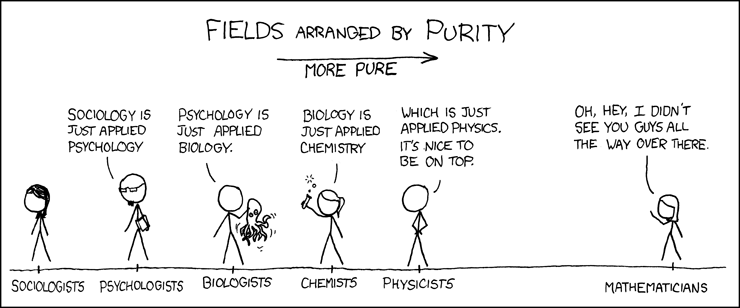
\includegraphics[scale = 0.45]{images/purity.png}\\
% 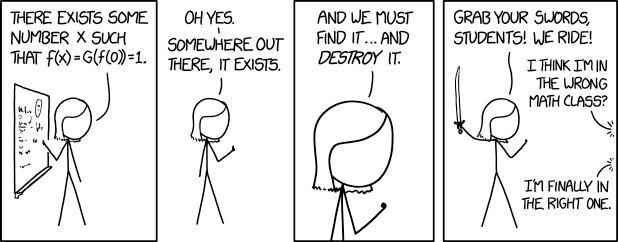
\includegraphics[scale = 0.55]{existence_proof}

% \chapter{Danksagung}

% \hl{Lorem ipsum dolor sit amet, consectetur adipiscing elit. Pellentesque vulputate pellentesque nunc, ut iaculis purus ornare nec. Nunc finibus rhoncus odio, non maximus tortor elementum eu. Duis rutrum tincidunt dignissim. Donec vel urna non felis congue iaculis. Aenean eu velit sagittis, tempor magna eu, volutpat urna. Integer lectus neque, auctor vitae eleifend quis, ullamcorper eu elit.}